\hypertarget{day-9---ux7f16ux5199-api}{%
\subsection{Day 9 - 编写 API}\label{day-9---ux7f16ux5199-api}}

自从 Roy Fielding 博士在 2000 年他的博士论文中提出
\href{http://zh.wikipedia.org/wiki/REST}{REST}(Representational State
Transfer)风格的软件架构模式后,REST 就基本上迅速取代了复杂而笨重的
SOAP,成为 Web API 的标准了。

什么是 Web API 呢?

如果我们想要获取一篇
Blog,输入\texttt{http://localhost:9000/blog/123},就可以看到 id
为\texttt{123}的 Blog 页面,但这个结果是 HTML 页面,它同时混合包含了
Blog 的数据和 Blog
的展示两个部分。对于用户来说,阅读起来没有问题,但是,如果机器读取,就很难从
HTML 中解析出 Blog 的数据。

如果一个 URL 返回的不是 HTML,而是机器能直接解析的数据,这个 URL
就可以看成是一个 Web
API。比如,读取\texttt{http://localhost:9000/api/blogs/123},如果能直接返回
Blog 的数据,那么机器就可以直接读取。

REST 就是一种设计 API 的模式。最常用的数据格式是 JSON。由于 JSON
能直接被 JavaScript 读取,所以,以 JSON 格式编写的 REST 风格的 API
具有简单、易读、易用的特点。

编写 API 有什么好处呢?由于 API 就是把 Web App
的功能全部封装了,所以,通过 API
操作数据,可以极大地把前端和后端的代码隔离,使得后端代码易于测试,前端代码编写更简单。

一个 API 也是一个 URL
的处理函数,我们希望能直接通过一个\texttt{@api}来把函数变成 JSON 格式的
REST API,这样,获取注册用户可以用一个 API 实现如下:

\begin{pythoncode}
@get('/api/users')
def api_get_users(*, page='1'):
    page_index = get_page_index(page)
    num = yield from User.findNumber('count(id)')
    p = Page(num, page_index)
    if num == 0:
        return dict(page=p, users=())
    users = yield from User.findAll(orderBy='created_at desc', limit=(p.offset, p.limit))
    for u in users:
        u.passwd = '******'
    return dict(page=p, users=users)
\end{pythoncode}

只要返回一个\texttt{dict},后续的\texttt{response}这个\texttt{middleware}就可以把结果序列化为
JSON 并返回。

我们需要对 Error 进行处理,因此定义一个\texttt{APIError},这种 Error
是指 API 调用时发生了逻辑错误(比如用户不存在),其他的 Error 视为
Bug,返回的错误代码为\texttt{internalerror}。

客户端调用 API 时,必须通过错误代码来区分 API
调用是否成功。错误代码是用来告诉调用者出错的原因。很多 API
用一个整数表示错误码,这种方式很难维护错误码,客户端拿到错误码还需要查表得知错误信息。更好的方式是用字符串表示错误代码,不需要看文档也能猜到错误原因。

可以在浏览器直接测试
API,例如,输入\texttt{http://localhost:9000/api/users},就可以看到返回的
JSON:

 
 \begin{figure}[htp]
	\centering
	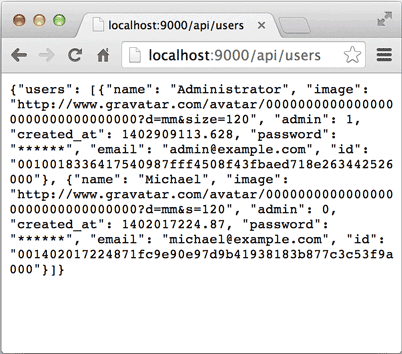
\includegraphics[width=0.6\linewidth]{fig/955712165379744.png}
\end{figure}


\hypertarget{ux53c2ux8003ux6e90ux7801}{%
\subsubsection{参考源码}\label{ux53c2ux8003ux6e90ux7801}}

\href{https://github.com/michaelliao/awesome-python3-webapp/tree/day-09}{day-09}

